\subsubsection{Example: Math achievement and SES}

To illustrate, we use a classic data set from %Bryk \& Raudenbush (2002)
\citet{BrykRaudenbush:1992} and \citet{RaudenbushBryk:2002}
dealing with math achievement scores for a subsample of 7,185 students from 160 schools
in the 1982 High School \& Beyond survey of U.S. public and Catholic high
schools conducted by the National Center for Education Statistics (NCES).
The data set contains 90 public schools and 70 Catholic schools, with
sample sizes ranging from 14 to 67.

The response is a standardized measure of math achievement, while
student-level predictor variables include sex and student socioeconomic status (SES), and
school-level predictors include sector (public or Catholic) and mean SES for the
school (among other variables).
Following \citet{RaudenbushBryk:2002}, student SES is considered the main predictor, and is
typically analyzed in centered within schools,
$\mathrm{CSES}_{ij} = \mathrm{SES}_{ij} - \mathrm{(mean SES)}_i$, for ease of interpretation (making the within-school intercept for school $i$
equal to the mean SES in that school).



\begin{figure}[htb]
 \begin{minipage}[b]{.49\linewidth}
  \centering
  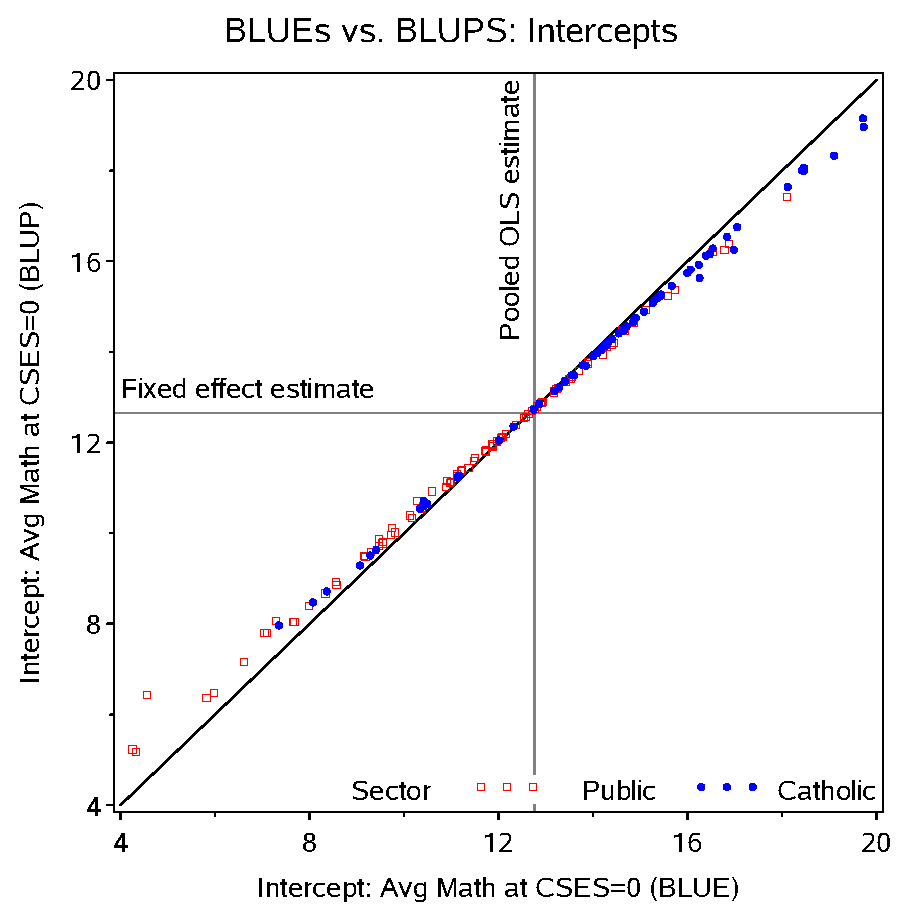
\includegraphics[width=1\linewidth,clip]{fig/hsbmix41}
%  \caption{}%
%  \label{fig:}
 \end{minipage}%
 \hfill
 \begin{minipage}[b]{.49\linewidth}
  \centering
  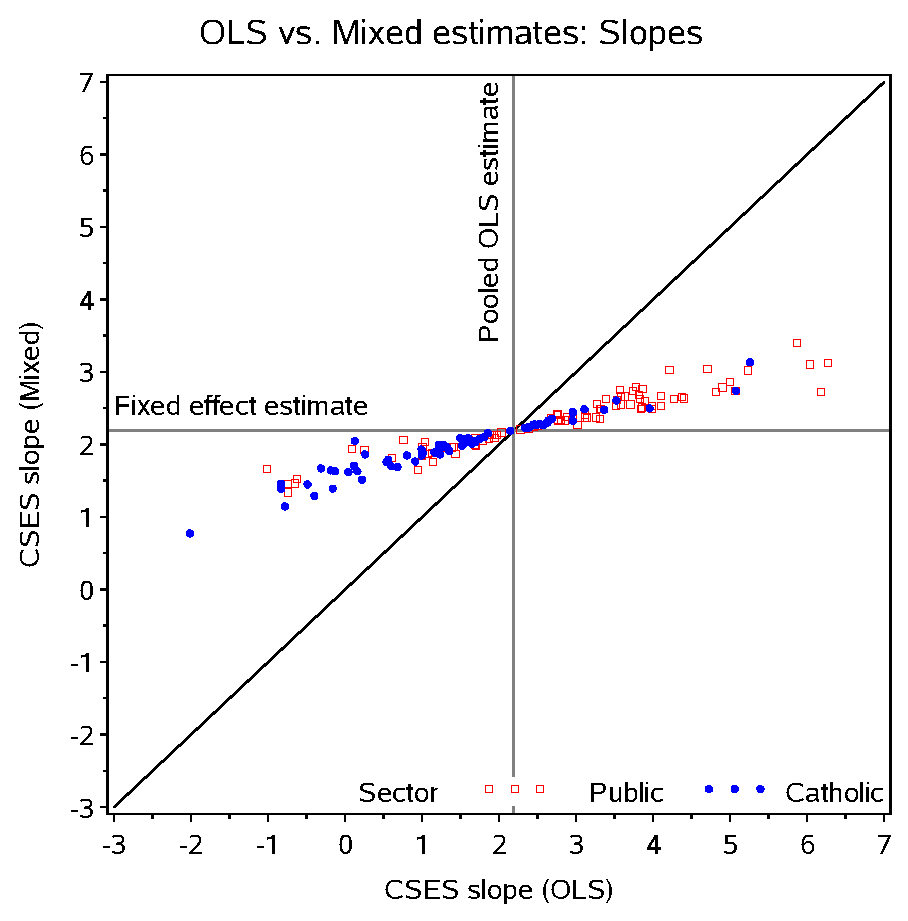
\includegraphics[width=1\linewidth,clip]{fig/hsbmix42}
 \end{minipage}
  \caption{Comparing BLUEs and BLUPs. Each panel plots the OLS estimates from separate regressions for each school (BLUEs)
  versus the mixed model estimates from the random intercepts and slopes model (BLUPs).
  Left: intercepts; Right: slopes for CSES.  The shrinkage of the BLUPs toward the OLS estimate is much greater for slopes than
  intercepts. }
  \label{fig:hsbmix4}
\end{figure}

For simplicity, we consider the case of CSES as
a single quantitative predictor in $\mat{X}$ in the example below.  We fit and compare the following models:
\begin{eqnarray}
 \vec{y}_{i} & \sim & \mathcal{N} ( \beta_0 + x_{i} \beta_1 + \epsilon_{i}  , \sigma^2 ) \quad\quad \textrm{pooled OLS} \\
 \vec{y}_{i} & \sim & \mathcal{N} ( \beta_{0i} + x_{i} \beta_{1i} + \epsilon_{i}  , \sigma^2_i ) \quad\quad \textrm{unpooled BLUEs} \\
 \vec{y}_{i} & \sim & \mathcal{N} ( \beta_{0i} + x_{i} \beta_{1i} + u_{0i} + x_{i} u_{1i} + \epsilon_{i}  , \sigma^2_i ) \quad\quad \textrm{random intercepts and slopes}
%
\end{eqnarray}
and also include a fixed effect of sector, common to all models; for compactness, the sector effect is elided in the notation above.

In expositions of mixed-effects models, such models are often compared visually by plotting predicted values in data space, where each school appears
as a fitted line under one of the models above (sometimes called ``spaghetti plots'').
Our geometric approach leads us to consider the equivalent but simpler plots in the dual $\beta$ space,
where each school appears as a point.

\figref{fig:hsbmix4} plots the unpooled BLUE estimates against those from the random effects model, with separate panels for intercepts
and slopes to illustrate the shrinkage of different parameters.  In these data, the variance in intercepts (average math achievement
for students at $\mathrm{CSES}=0$), $g_{00}$,
among schools in each sector is large, so the mixed effects estimates have small weight and there is little
shrinkage.  On the other hand, the variance component for slopes, $g_{11}$, is relatively small, so there is greater
shrinkage toward the BLUE, fixed effect estimates.

\begin{figure}[htb!]
  \centering
  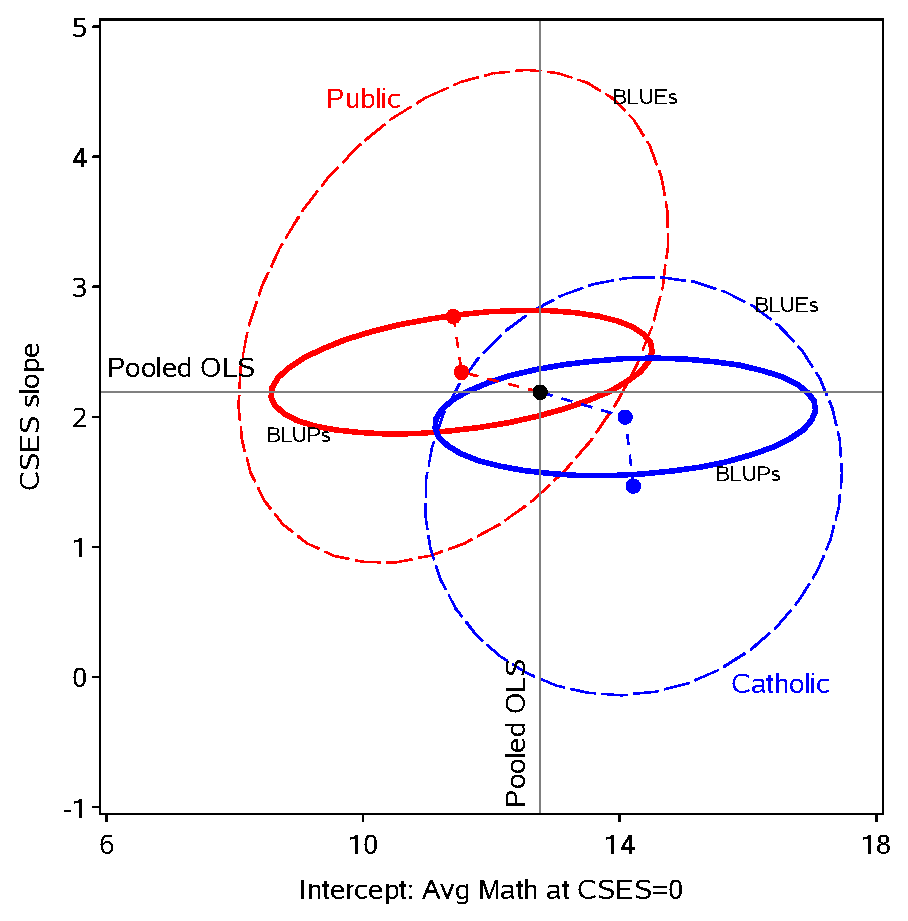
\includegraphics[width=.6\textwidth,clip]{fig/hsbmix43}
  \caption{Comparing BLUEs and BLUPs. The plot shows ellipses of 50\% coverage for the estimates of intercepts and slopes
  from OLS regressions (BLUEs) and the mixed model (BLUPs), separately for each sector.
  The centers of the ellipses illustrate how the BLUPS can be considered a weighted average of the BLUEs and the
  pooled OLS estimate, ignoring sector. The relative sizes of the ellipses reflect the smaller variance for the
  BLUPs compared to the BLUEs, particularly for slope estimates. }%
  \label{fig:hsbmix43}
\end{figure}

For the present purposes, a more useful visual representation of these model comparisons can be shown together in
the space of $(\beta_0, \beta_1)$, as in \figref{fig:hsbmix43}.  Estimates for individual schools are not shown,
but rather these are summarized by the ellipses of 50\% coverage for the BLUEs and BLUPs within each sector.
The centers of the ellipsoids indicate the relatively greater shrinkage of slopes compared to intercepts.
The sizes of ellipsoids show directly the greater precision of the BLUPs, particularly for slopes.
